\label{sec:dataset}

While conducting the experiment, we noticed some deviations with the reported dataset, and we include some basic exploratory data analysis (EDA) to offer a comprehensive overview of the dataset.
The \texttt{PTB–XL} dataset provides us with \texttt{records100}, a downsampled version of \texttt{records500}; however, for sake of reproducibility and comparison fairness,
we confine ourselves to \texttt{records100}. Furthermore, for sake of memory usage and computing purposes, we shall reduce to data from \texttt{float64} to \texttt{float32}.
Also, this section serves as an agreement on the dataset used in the modelling pipeline to compare between the reproduced and our results.
Firstly, let us discuss the target classes or diagnostic labels/classes, and the ECG signals thereafter. Details presented herein is extracted from the \texttt{eda.ipynb} in our repository.

For the diagnostic labels, they annotated the dataset with 24 subclasses and further grouped into 5 superclasses, by the help of at most two cardiologists. 
An illustration is given as below.

\begin{figure}[H]
    \centering
    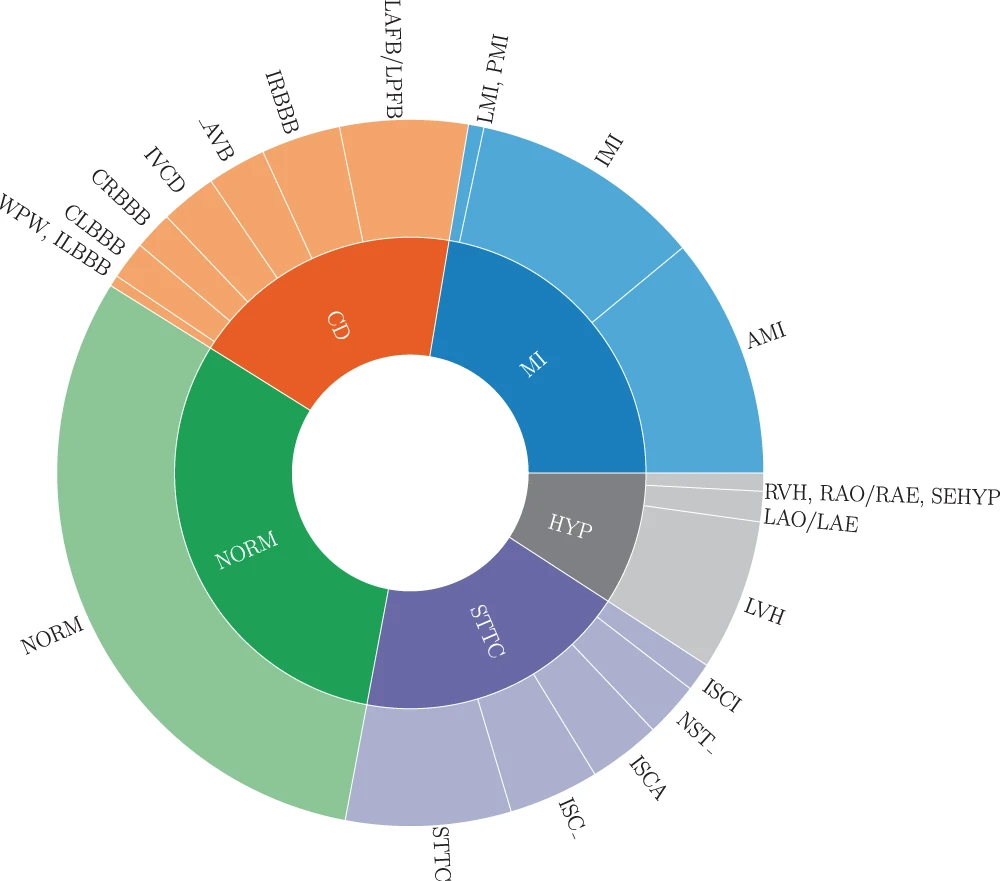
\includegraphics[width=0.7\textwidth]{figures/intro_eda/classes.png}
    \caption{Graphical summary of superclasses and their subclasses, adopted from \cite{wagner2020ptbxl}.}
    \label{fig:super_sub_visual}
\end{figure}

Let us first present the distribution of data w.r.t the diagnostic superclasses. We omit the description of what superclass acronyms stand for, as one can work without knowing.

\begin{figure}[H]
    \centering
    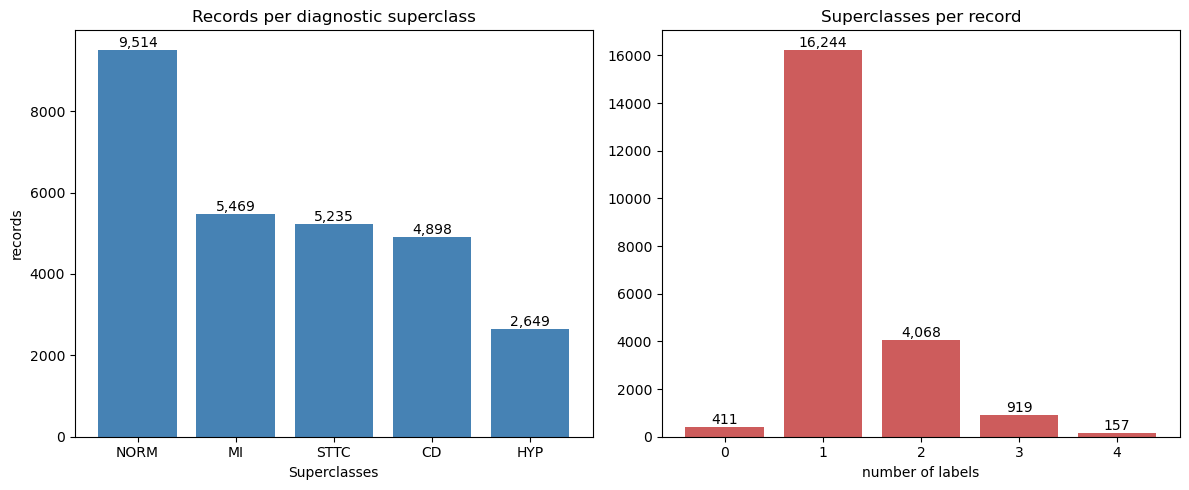
\includegraphics[width=0.95\textwidth]{figures/intro_eda/raw_class_distribution.png}
    \caption{Distribution of the diagnostic superclasses over the \texttt{records100} subset of \texttt{PTB–XL}.
    \textbf{Left:} the number of records carrying each superclass.
    \textbf{Right:} the number of superclasses assigned to each record.}
    \label{fig:class_distribution}
\end{figure}

As described in the original paper, we are working with a multiclass, not multilabel, classification task, and thus, they only considered records annotated with one label and dropped all recorded without annotations.
For brevity, we shall refer to 1–label (multiclass) dataset as ``dataset'', unless stated otherwise.
We present data distribution as below.

\begin{figure}[H]
    \centering
    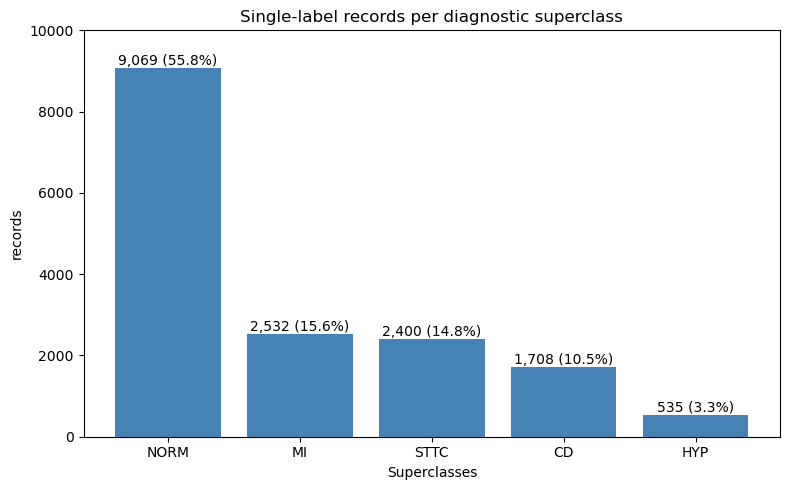
\includegraphics[width=0.7\textwidth]{figures/intro_eda/label_1_distribution.png}
    \caption{Distribution of the single diagnostic superclass over the \texttt{records100} subset of \texttt{PTB–XL}}
    \label{fig:1_class_distribution}
\end{figure}

Next, let us investigate the ECG records. In brief, each ECG record has a shape of $(1000 \times 12)$, where $1000$ represents the number of samples within 10 seconds, and $12$ implies the number of leads used in the clinical study.
Let us illustrate the first ECG record in the dataset as follows.

\begin{figure}[H]
    \centering
    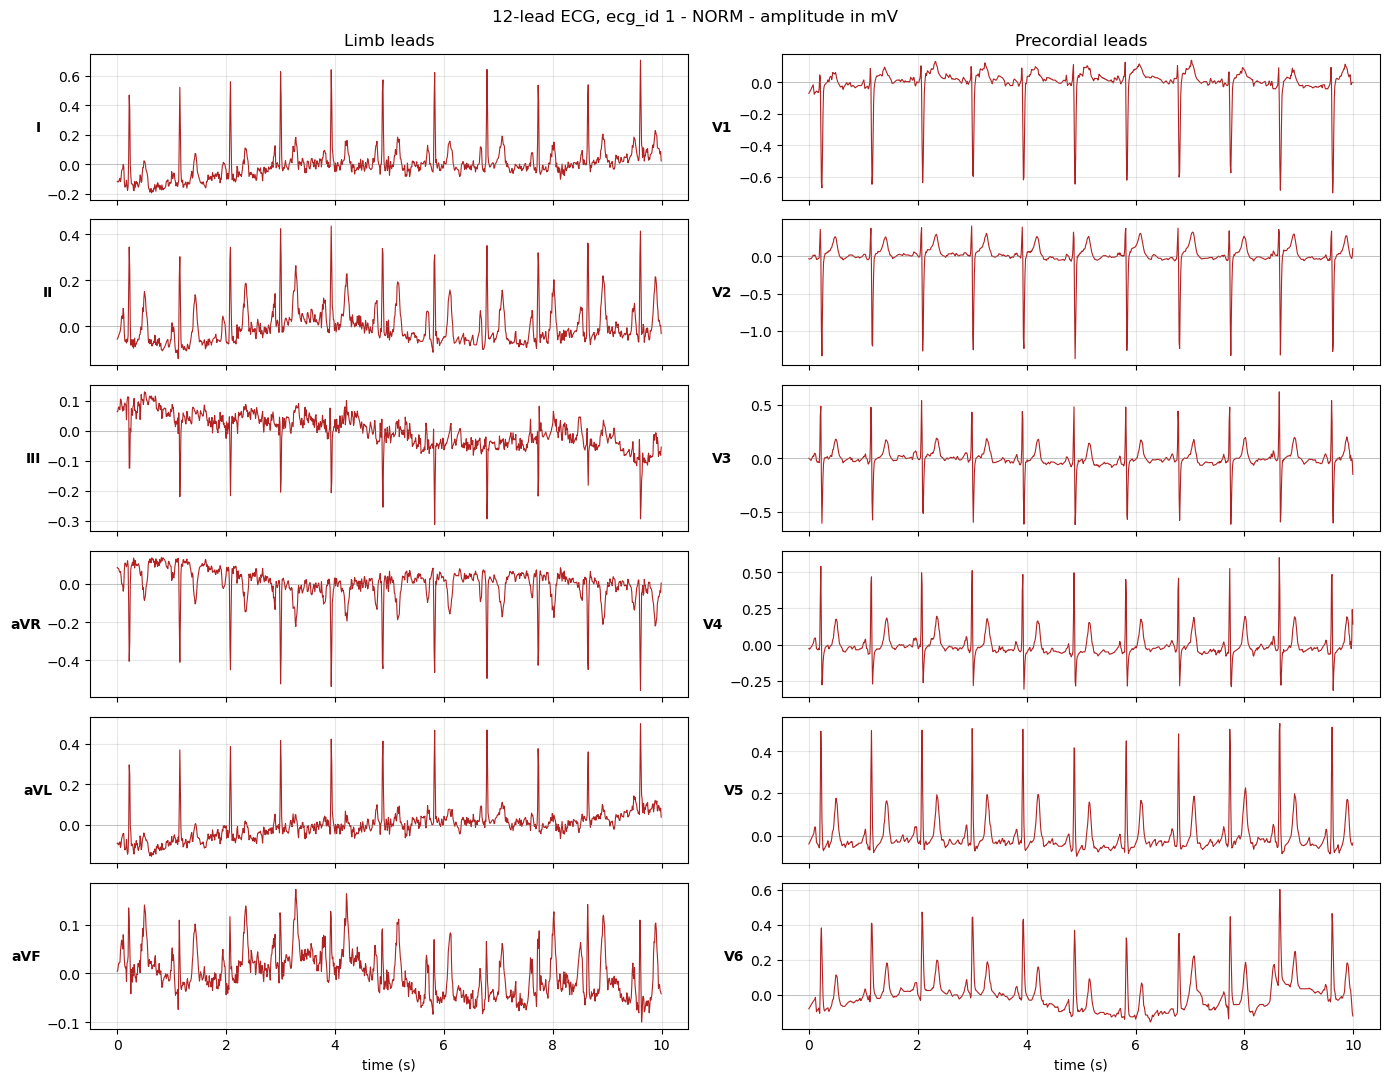
\includegraphics[width=1\textwidth]{figures/intro_eda/leads_visuals.png}
    \caption{12-lead ECG visualisation.}
    \label{fig:12_lead_ecg}
\end{figure}

Next, let us verify if there are missing values in the dataset. We verify if there are any \texttt{NaN}/\texttt{Inf} in the records, also, if any ECG record shows zero variance, this may be subject to sensor errors, and treated as missing values.
Let us demonstrate the distribution of the ECG signals w.r.t all 12 leads as follows.

\begin{figure}[H]
    \centering
    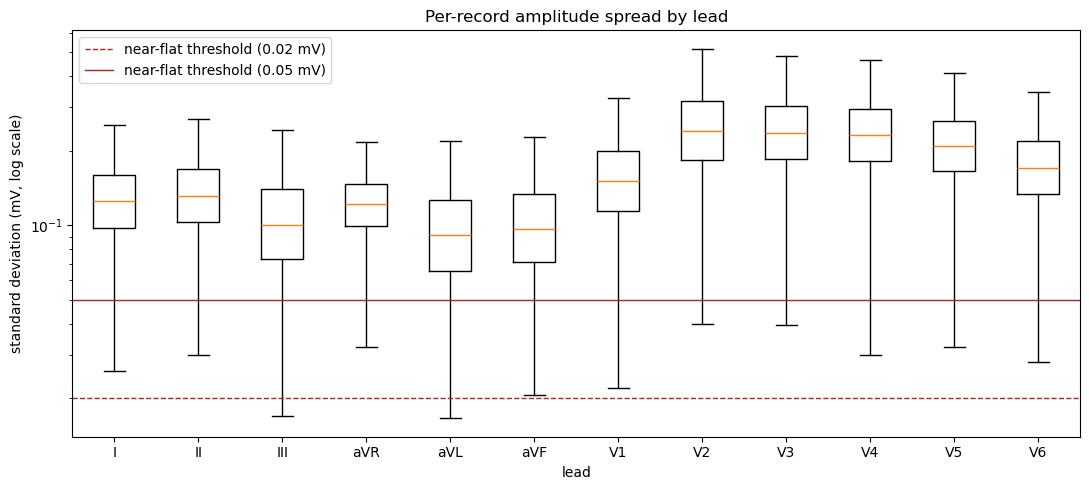
\includegraphics[width=0.7\textwidth]{figures/intro_eda/amplitude_std.png}
    \caption{Per–record amplitude standard deviation.}
    \label{fig:amplitude_spread}
\end{figure}

More thoroughly, there are no missing values presented; still, many ECG records comprise of low–variance signals, which might be recorded from CVD patients.

\begin{table}[H]
    \centering
    \caption{Near–flat leads and the records containing them, at increasing thresholds on the per–lead amplitude standard deviation $\sigma$.}
    \label{tab:near_flat_leads}
    \begin{tabular}{lrr}
        \toprule
        Threshold & Near–flat leads & Affected records \\
        \midrule
        $\sigma < 0.005$ mV & $0$     & $0$     \\
        $\sigma < 0.010$ mV & $0$     & $0$     \\
        $\sigma < 0.020$ mV & $5$     & $5$     \\
        $\sigma < 0.050$ mV & $4{,}119$ & $3{,}416$ \\
        \bottomrule
    \end{tabular}
\end{table}
